\chapter{Discussion}\label{chp6:discussion}

In this chapter we will discuss the viability of the low frequency acoustic emanations, and how current guidelines for shielding information systems are helping in protecting against this potential threat.
We will also look at the cost involved in building a setup able to process these emanations, and the implications of this.
Last, we will look at use cases where the analysis of these emanations will be useful.

\section{Viability of Extracted Information}
We have not obtained a basis for drawing a conclusion as to whereas the emanations as presented in the previous chapters are in fact caused by the \gls{CPU}.
However, we have tried to capture the effect at different positions on our Lenovo T60p laptop. 
For this specific computer we experienced that it is far easier to find the patterns we are looking for in the resulting power spectra when the recordings are done right above the \gls{CPU}.
We also found that slight disposition of the microphone, still hovering the \gls{CPU} cooling block, notably impact the signal strength.


\section{Significance of Results}
Using the acoustic side channel, we are able to distinguish between the MEM operation and the other microinstruction loops.
The results given in~\cite[Fig.~2]{DBLP:conf/crypto/GenkinST14} suggest that it is possible to observe a difference, even between the different microinstructions ADD, MUL and NOP. 
The most visible difference is in a frequency range much higher than the hard limit imposed on us by the sampling rate of our setup.
Results given here are therefore inconclusive when it comes down to distinguishing between the NOP, MUL and ADD instructions.
~\autoref{fig:T60p-knowles-micro-ips-0}

We have conducted experiments using different configurations of hardware and observe big variations in acoustic fingerprints for the different computers, as seen in~\autoref{fig:comparison_micorinstructions}.
An interesting side note is how the acoustic emanations of the Lenovo T60p laptop is changing depending on if the computer is running on battery power (\autoref{fig:comparison_T60p-ekkofritt-bk-micro-ips-3}) or with a power adapter (\autoref{fig:comparison_T60p-ekkofritt-bk-micro-eps-1}).
The noise introduced by the power adapter is not emanating from the power adapter itself, as we have experimented with the positioning of the adapter, without seeing any impact on the resulting acoustic fingerprints.

We did not do any experiments to explore if the captured signals are in fact acoustic, or if they are caused by electromagnetic signals.

\begin{figure}[ht]
    \centering
    \begin{subfigure}{0.32\textwidth}
        \centering
        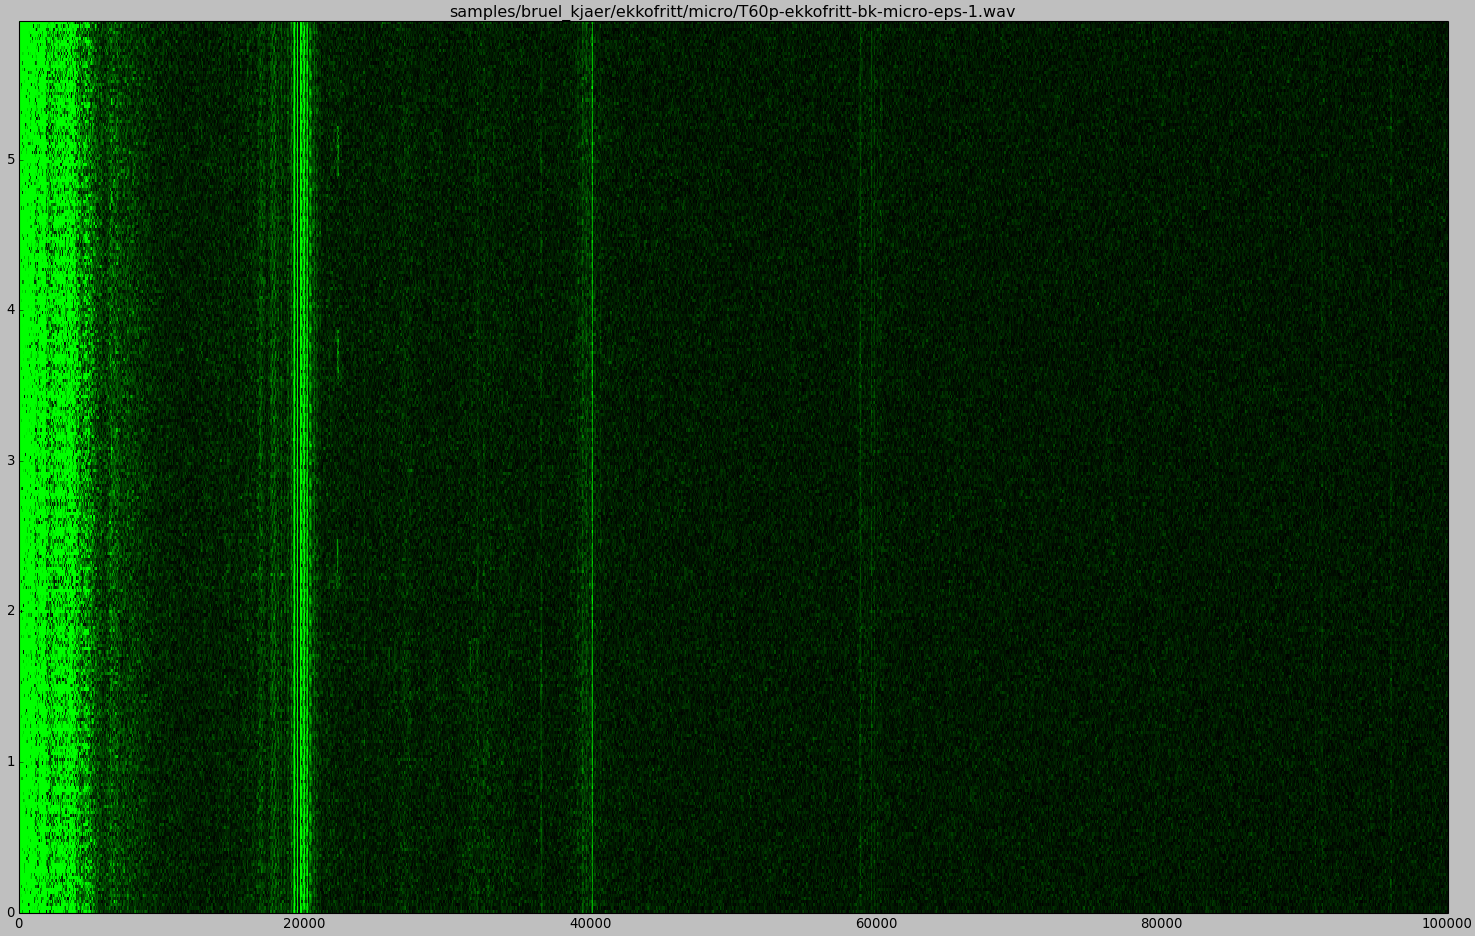
\includegraphics[width=1\linewidth]{T60p-ekkofritt-bk-micro-eps-1.png}
        \caption{Lenovo T60p}
        \label{fig:comparison_T60p-ekkofritt-bk-micro-eps-1}
    \end{subfigure}
    \begin{subfigure}{0.32\textwidth}
        \centering
        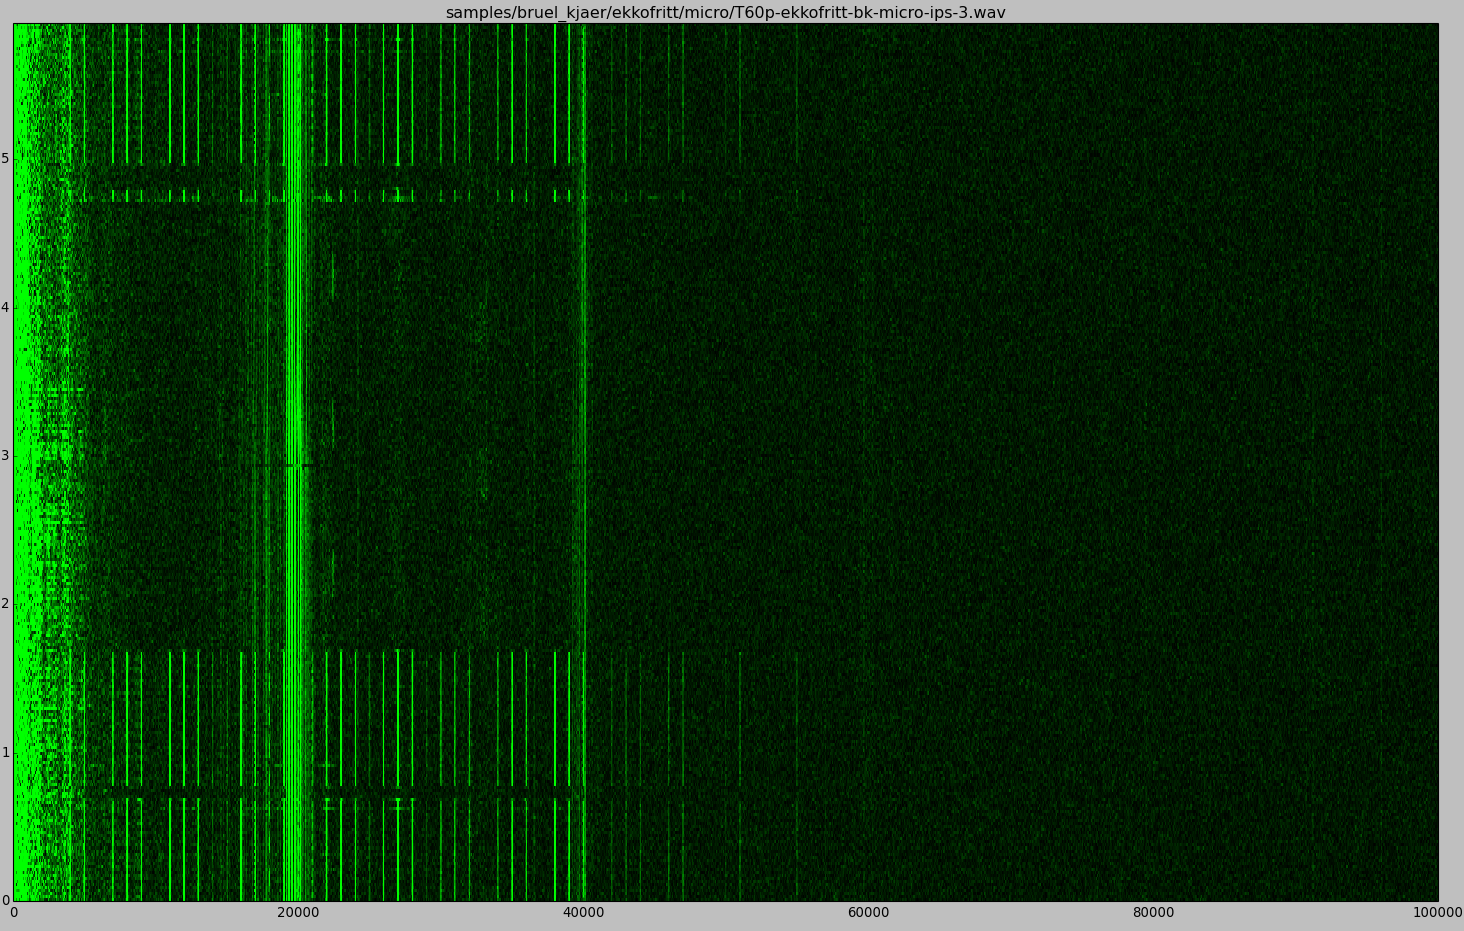
\includegraphics[width=1\linewidth]{T60p-ekkofritt-bk-micro-ips-3.png}
        \caption{Lenovo T60p}
        \label{fig:comparison_T60p-ekkofritt-bk-micro-ips-3}
    \end{subfigure}
    \begin{subfigure}{0.32\textwidth}
        \centering
        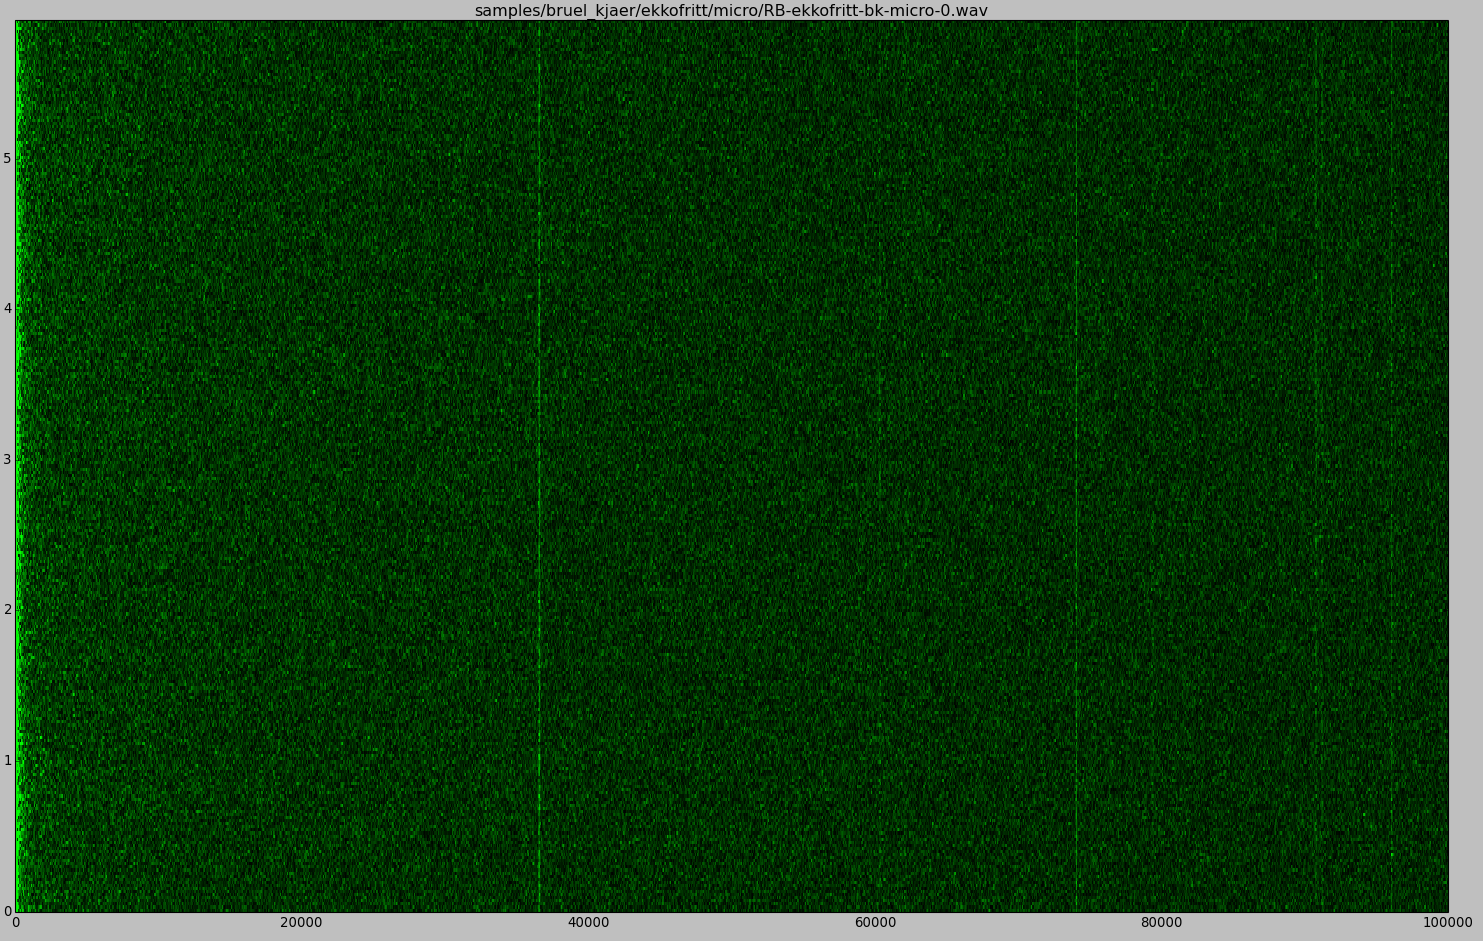
\includegraphics[width=1\linewidth]{RB-ekkofritt-bk-micro-0.png}
        \caption{Raspberry PI}
        \label{fig:comparison_RB-ekkofritt-bk-micro-0}
    \end{subfigure}
    \begin{subfigure}{0.32\textwidth}
        \centering
        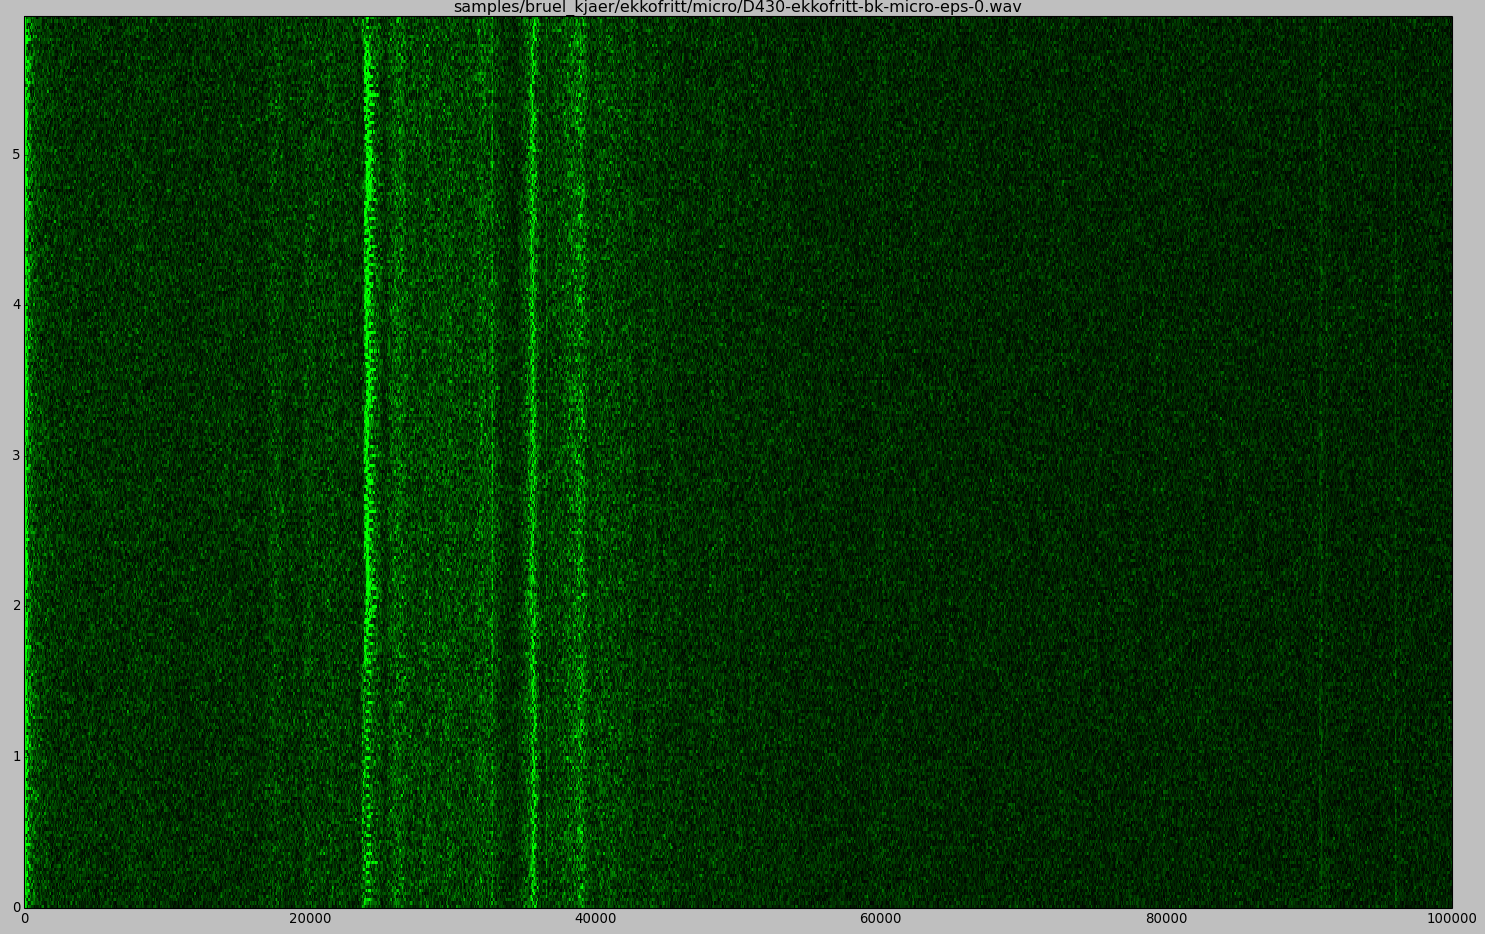
\includegraphics[width=1\linewidth]{D430-ekkofritt-bk-micro-eps-0.png}
        \caption{Dell 430}
        \label{fig:comparison_D430-ekkofritt-bk-micro-eps-0}
    \end{subfigure}
    \begin{subfigure}{0.32\textwidth}
        \centering
        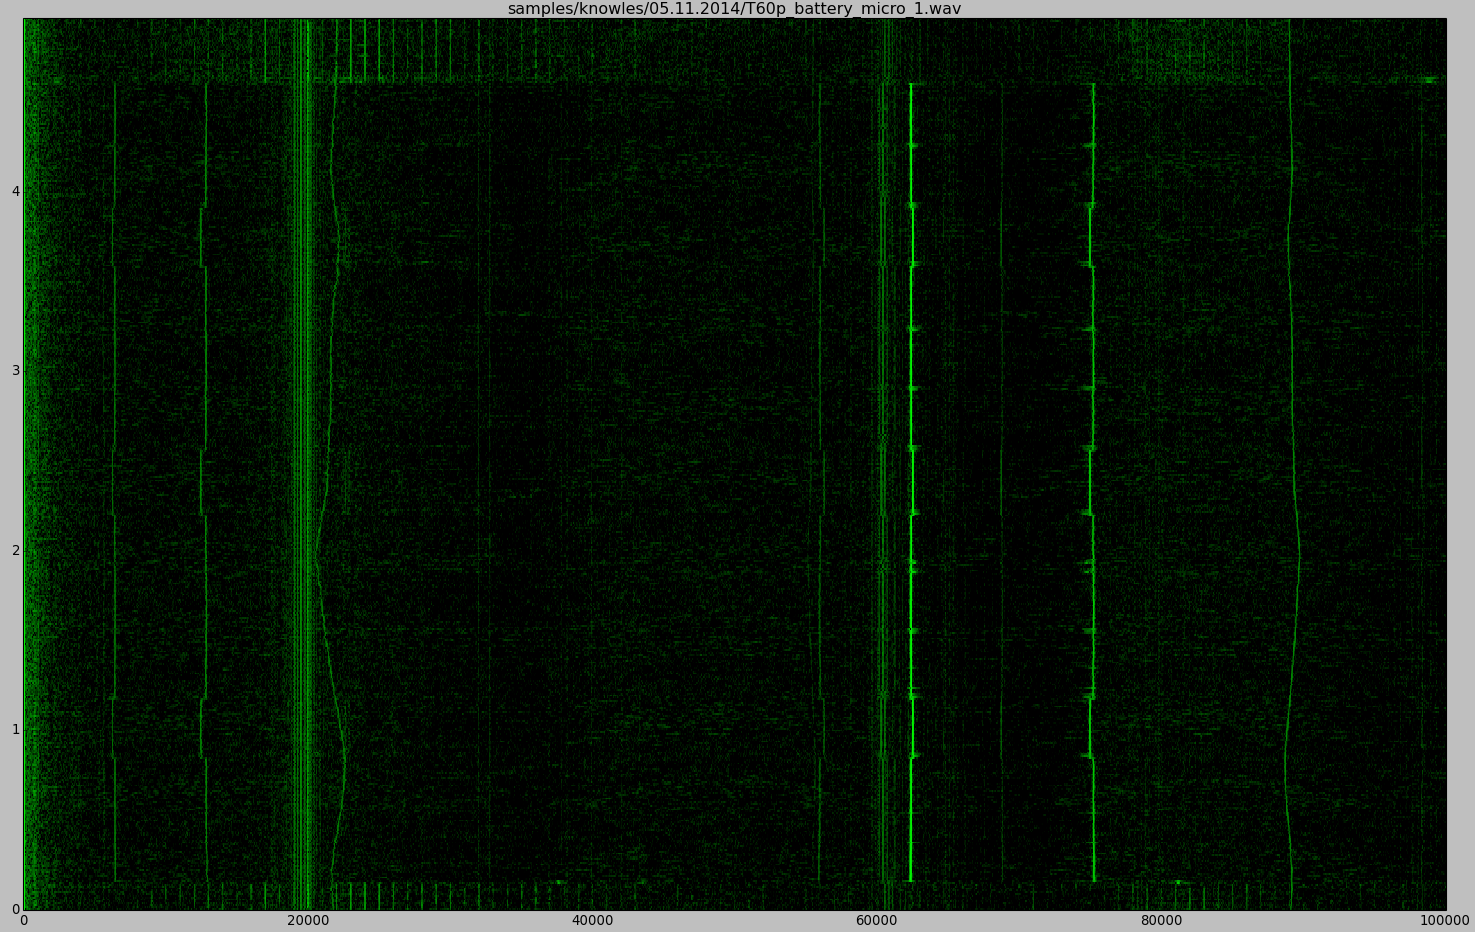
\includegraphics[width=1\linewidth]{T60p-knowles-micro-ips-0.png}
        \caption{Lenovo T60p}
        \label{fig:comparison_T60p-knowles-micro-ips-0}
    \end{subfigure}
    \begin{subfigure}{0.32\textwidth}
        \centering
        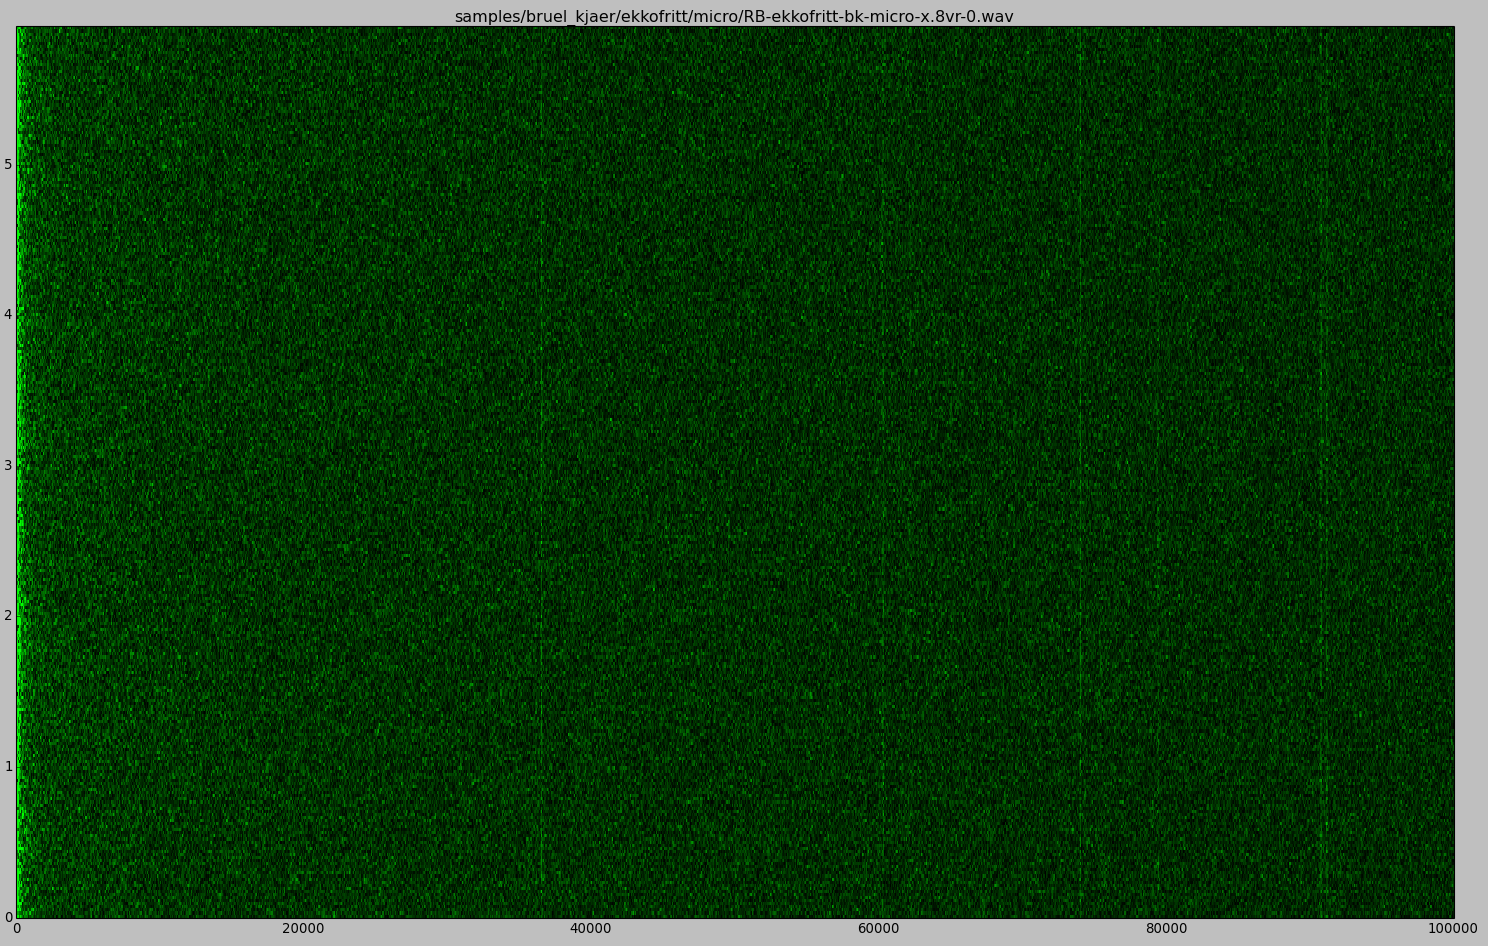
\includegraphics[width=1\linewidth]{RB-ekkofritt-bk-micro-x-8vr-0.png}
        \caption{Raspberry PI}
        \label{fig:comparison_RB-ekkofritt-bk-micro-x-8vr-0}
    \end{subfigure}
    \caption{ Acoustic emanations when performing the microinstructions on following devices:
    (a) T60p with Brüel\&Kjær running on power adopter.
    (b) T60p with Brüel\&Kjær running on battery power.
    (c) Raspberry PI on CPU with Brüel\&Kjær.
    (d) Dell D430 with Brüel\&Kjær running on battery power.
    (e) T60p with Knowles running on battery power.
    (f) Raspberry PI on power with Brüel\&Kjær.}
    \label{fig:comparison_micorinstructions}
\end{figure}

\section{Analysis Beyond Extremes}
In our experiments, we were able to distinguish between different extremes in \gls{CPU} activity based strictly on acoustic leakage. 
We do not use any mathematical models, but rely on empirical analysis of the power spectra. 
This is a limiting factor in the sense that we are only able to draw conclusions based on clear patterns in the resulting data that are visible to the human eye, when presented in the way done here and by Genkin et al.
None of the experiments we performed included real time analysis of the leakage, hence we were limited to look for patterns resulting from static programs being executed, to be able to relate the information captured to the time domain in our offline analysis.
Real time analysis, together with mathematical models for correlation, would allow a more statistical approach to distinguishing between distinct fingerprints, and could allow for attacks along the line of what is proposed in~\cite{DBLP:conf/crypto/KocherJJ99}, only using acoustic emanations rather than power traces for analysis.


\section{ARM Processors and Possible Attack Vectors}
We chose to conduct experiments on a Lenovo laptop computer similar to what is used by Genkin et al., and also on an even older Dell laptop, as it was suggested that older processors had more explicit acoustic fingerprints.
In addition, we conducted the same experiments for a Raspberry Pi, which is equipped with an ARM \gls{CPU}.

A motivation for looking at ARM processors is that a lot of electronic equipment today is running on the ARM architecture.
The potential of analyzing network traffic by looking at routers is just one of several interesting approaches to exploit the potential of low frequency acoustic emanations.
Unfortunately, we found it much harder to distinguish between operations on the Raspberry Pi, than for the laptops running on x86/x64 Intel processors.
It is still worth noting that the findings of Genkin et al. suggest that distinguishing between different RSA keys used for decryption can be done using this side channel; in the case of a router, this means that the approach could be a viable way to analyze ongoing IPSec sessions, where the router performs encryption or decryption, without being connected to the network at all.


\section{Possible Attack Scenarios}\label{chp6:sec:attack_scenarios}


\section{Applicability}\label{chp6:sec:applicability}

Red/Black Engineering-Installation Guidelines~\cite{MIL_HDBK_232} created by the Department of Defence, Washington DC, states in 30.1 page 91 that unauthorized (BLACK) and authorized (RED) equipment should at least be separated with 3 feet / 0.9m. 
Other electronic devices such as mobile phones and personal laptops should not be permitted to areas where RED equipment is installed. 

In the guidance paper about protection against eavesdropping~\cite{NSM_avlytting} published by Norges Sikkerhetsmyndigheter (NSM), it is recommended in section 9-8 (page 7) that one should follow the TEMPEST guidance when installing an informationsystem.

\section{Future Work}\label{chp6:sec:future_work}
\begin{enumerate}
	\item ADD loops of different lengths
	\item Statistical models for correlation
	\item Real time analysis
	\item Experiments on the proposed attack against RSA
	\item Listening to GPU for reproducing display
\end{enumerate}